\documentclass[border={0.1cm 0.1cm 0.1cm 0.1cm}]{standalone}  %E,S,W,N

\usepackage{amssymb}
\usepackage{amsmath}
\usepackage{tikz}

\begin{document}
	
	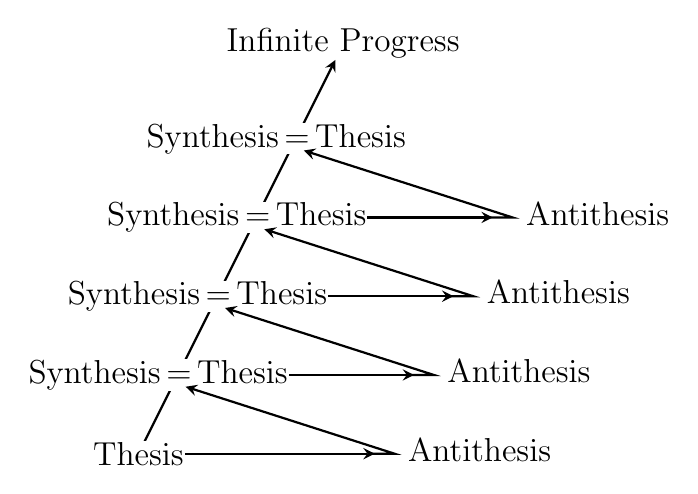
\begin{tikzpicture}[thick]
	\def\n{3} %original: n=3
	\node[fill=white,inner sep=0.3,above] at ({0.5*(\n+2)+0.1},\n+2) {\large Infinite Progress};
	\draw[->,>=stealth] (0,0)--({0.5*(\n+2)},\n+2);
	%\draw ({0.5*(\n+1)},\n+1)--({0.5*(\n+2)},\n+1); %last Thesis
	
	\foreach \i in {\n,...,0}{
	%\node[left] at (0.4+0.5*\i,1+\i) {\large Synthesis};
	%\node[right,fill=white,inner sep=0.3] at (0.75+0.5*\i,1.05+\i) {\large Thesis};
	\node[fill=white,inner sep=0.3] at (0.25+0.5*\i,1+\i) {\large Synthesis$\,$=$\,$Thesis};
	\draw[->,>=stealth] (0.5*\i,\i)--(0.5*\i+3,\i);
	\draw[->,>=stealth] (0.5*\i+3-0.05,\i)--(0.5*\i+3.25,\i)--(0.6+0.5*\i,\i+0.85);
	\node[right,fill=white,inner sep=0.3] at (0.5*\i+3.4,0.05+\i) {\large Antithesis};
	}
	
	\node[fill=white,inner sep=0.3] at (0,0) {\large Thesis}; %bottom thesis
	\end{tikzpicture}
	
\end{document}